% !TEX root = ../Thesis.tex
\chapter{Trap-Driven Simulation}

Because superpage overlays require hardware changes, they can only be tested in a simulated system. To allow us to simulate superpage overlays in real time on real workloads, we use a system called trap-driven simulation \cite{Talluri}. This is an alternative to trace-driven simulation, where the workload's memory accesses are logged and processed after the benchmark is done to measure how the simulated system would have performed. In contrast, trap-driven simulation runs the simulation in the operating system while the benchmark executes. It is generally faster and more flexible than trace-driven simulation, because not every memory access invokes overhead and the simulation has real-time kernel-level access to the system \cite{Uhlig}.

\section{Design}
The trap-driven simulation framework we developed is similar to the Tapeworm II system presented in 1994 \cite{Uhlig}, but running in a modern Linux kernel on x86-64. The kernel keeps track of a simulated TLB while the workload runs, and page tables are modified to force a page fault to occur on every memory access that would be a miss in the simulated TLB. The simulation can thus reliably be updated to reflect the correct TLB state.

An existing system called BadgerTrap \cite{BadgerTrap} was used as the basis of our infrastructure. BadgerTrap measures real TLB misses by a method similar to trap-driven simulation. Each page table entry in x86-64 has a section of ``reserved'' bits, which are not supposed to be touched by the software. When the MMU sees a reserved bit set during a page table walk, it immediately page faults with a specific error code. BadgerTrap takes advantage of this by setting a reserved bit on every page in the address space of the process being tested. Then, whenever there is a TLB miss the resulting page table walk causes a distinctive page fault, which BadgerTrap records. It proceeds to unset the reserved bit, read the address to get it into the TLB, and sets the reserved bit again. This means that the workload can continue running as normal, using the address translation in the TLB, but the next TLB miss will once again cause a page fault.

We ported BadgerTrap to version 4.6 of the Linux kernel and modified it to simulate a TLB. Every time an address is replaced in the simulated TLB, it is flushed from the real TLB as well so that every access that would be a miss in the simulation is also a miss in the real TLB. That allows the simulation to remain accurate to how a real system would behave under the same workload, and the performance impact is minimal since it only does any work on TLB misses.

Trap-driven simulation works as long as TLB misses are the only time any updates need to happen. The only thing this limits significantly is the replacement policy. We use a variant of ``not recently used'' (NRU), where a bit is set whenever the page is accessed, by also clearing pages from the real TLB if their ``used'' bit is 0 so that it can be updated on their next access. Pages with a 0 ``used'' bit are replaced first, and if all pages have it set then all the ``used'' bits are cleared and the first page is replaced.

\section{Evaluation}
The trap-driven simulation framework can be evaluated by comparing its results to the Linux \verb|perf| tool, which uses hardware counters to measure real TLB misses and other metrics. The correspondence is not exact for two reasons. First, the simulated TLB is not identical to the real one. For simplicity, we used only one level where the real system has L1 and L2 TLBs, and the size may not be exactly the same. Second, the simulation does not track kernel pages or the effects of context switches. The goal is simply to show that the simulation is a reasonable representation of how the TLB will be affected by various modifications.

To do this evaluation, we simply use a basic fork-write benchmark that allocates 2MB of memory as either one superpage or many regular pages, forks, and the child process writes to some part of the memory region. This triggers one or more copy-on-write, and the performance depends on how many TLB misses occur during the writes and how much data is copied.

\section{Results}

Figure \ref{fig:charts} shows simulated TLB misses vs real TLB misses measured by the \verb|perf| tool. The data is from a few different runs of the fork-write benchmark with different numbers of iterations. The simple linear relationship serves as a good sanity check showing that the trap-driven simulation is behaving similarly to the real TLB. The difference between simulated and real TLB misses is due to the differneces between the simulated and real system discussed above.

\begin{figure}
    \centering
    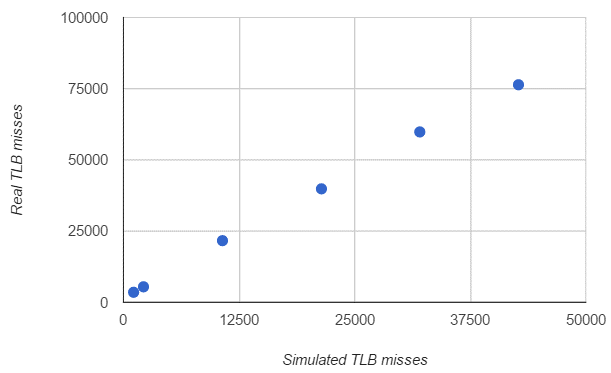
\includegraphics[width=3in]{Figures/Graph2}
    \caption{Simulated vs. real TLB misses on a simple benchmark}
    \label{fig:charts}
\end{figure}

\section{Conclusions}

In addition to being a good tool for evaluating superpage overlays, this trap-driven simulation framework can be useful for all kinds of TLB studies. It is very easy to change the size and associativity of the simulated TLB, and any special TLB behavior that would occur on a TLB miss can be implemented by modifying the miss handling code in the simulation.

As Uhlig \emph{et al.} point out, this system is preferable in many situations to the more common trace-driven simulation solutions\cite{Uhlig}. Simulations run relatively fast because only TLB misses causes overhead, and real-time access to kernel data structures allows more complicated modifications to be simulated. For example, in the overlay simulation the system splits superpages whenever an overlay is made, but keeps track of the pages that were split so that the simulation can act as if it was not split. This allows accesses to be tracked at small page granularity while still simulating a superpage.
